
\subsection{Mobility}

\textbf{Motivation.} Mobility in chess is a measure of the available moves a player can make in a given position. The idea is that if a player has more available moves, the position is stronger. In \cite{slater:1950} it was shown that there is a strong correlation between a player's mobility and the number of games won. This metric has been used extensively in handcrafted evaluations, and I propose to include this information as features for the neural network. \\

\textbf{Experiment.} There are two ways to go about encoding mobility:

\begin{itemize}
\item \textbf{Bitsets (per piece type):} Provide the exact squares each piece type can move to. The number of features would be $64 * 6 * 2 = 768$. The problem with this approach is not the amount of features, but the number of updates to the accumulator per move is very high, which slows down the search.

\begin{figure}[H]
\centering

\begin{tabular}{ccccc}

\raisebox{-7ex}{\chessboard[
    setfen=r5k1/1b1p1ppp/p7/1p1Q4/2p1r3/PP4Pq/BBP2b1P/R4R1K w - - 0 20,
    tinyboard,
    showmover=false,
]}
&

\raisebox{-7ex}{\chessboard[
    tinyboard,
    showmover=false,
    setwhite={ba2,bb2},
    pgfstyle=color,
    opacity=0.8,
    color=blue,
    markfield={b1,c1,c3,d4,e5,f6,g7}
]}

&

\raisebox{-7ex}{\chessboard[
    tinyboard,
    showmover=false,
    addblack={Bb7,Bf2},
    pgfstyle=color,
    opacity=0.8,
    color=blue,
    markfield={c8,c6,d5,a7,b6,c5,d4,e3,e1,g1,g3}
]}

&

\raisebox{-7ex}{\chessboard[
    tinyboard,
    showmover=false,
    setwhite={qd5},
    pgfstyle=color,
    opacity=0.8,
    color=blue,
    markfield={d6,d7,e6,f7,e5,f5,g5,h5,e4,d4,d3,d2,d1,c4,c5,b5,c6,b7}
]}

& $\hdots$

\\

Board &
\makecell{\white White\\\symbishop\ Bishop} &
\makecell{\black Black\\\symbishop\ Bishop} &
\makecell{\white White\\\symqueen\ Queen}

\end{tabular}
\end{figure}


\item \textbf{Counts (per piece type):} Use the number of available moves per piece type as features. This means having a feature for each possible count value, which are a lot less feature updates. To find which values to include as features I computed the total mobility for each piece role in 2 billion boards, shown in figure \ref{fig:mobility}. From the data, we can extract the range of values to use as features:

\begin{table}[H]
\centering
\begin{tabular}{c|c|c}
\toprule
\textbf{Piece role} & \textbf{Min} & \textbf{Max} \\
\midrule
\sympawn\ Pawn & 0 & 8+ \\
\symknight\ Knight & 0 & 15+ \\
\symbishop\ Bishop & 0 & 16+ \\
\symrook\ Rook & 0 & 25+ \\
\symqueen\ Queen & 0 & 25+ \\
\symking\ King & 0 & 8 \\
\bottomrule
\end{tabular}
\end{table}

\begin{figure}[H]
\centering
\makebox[\textwidth]{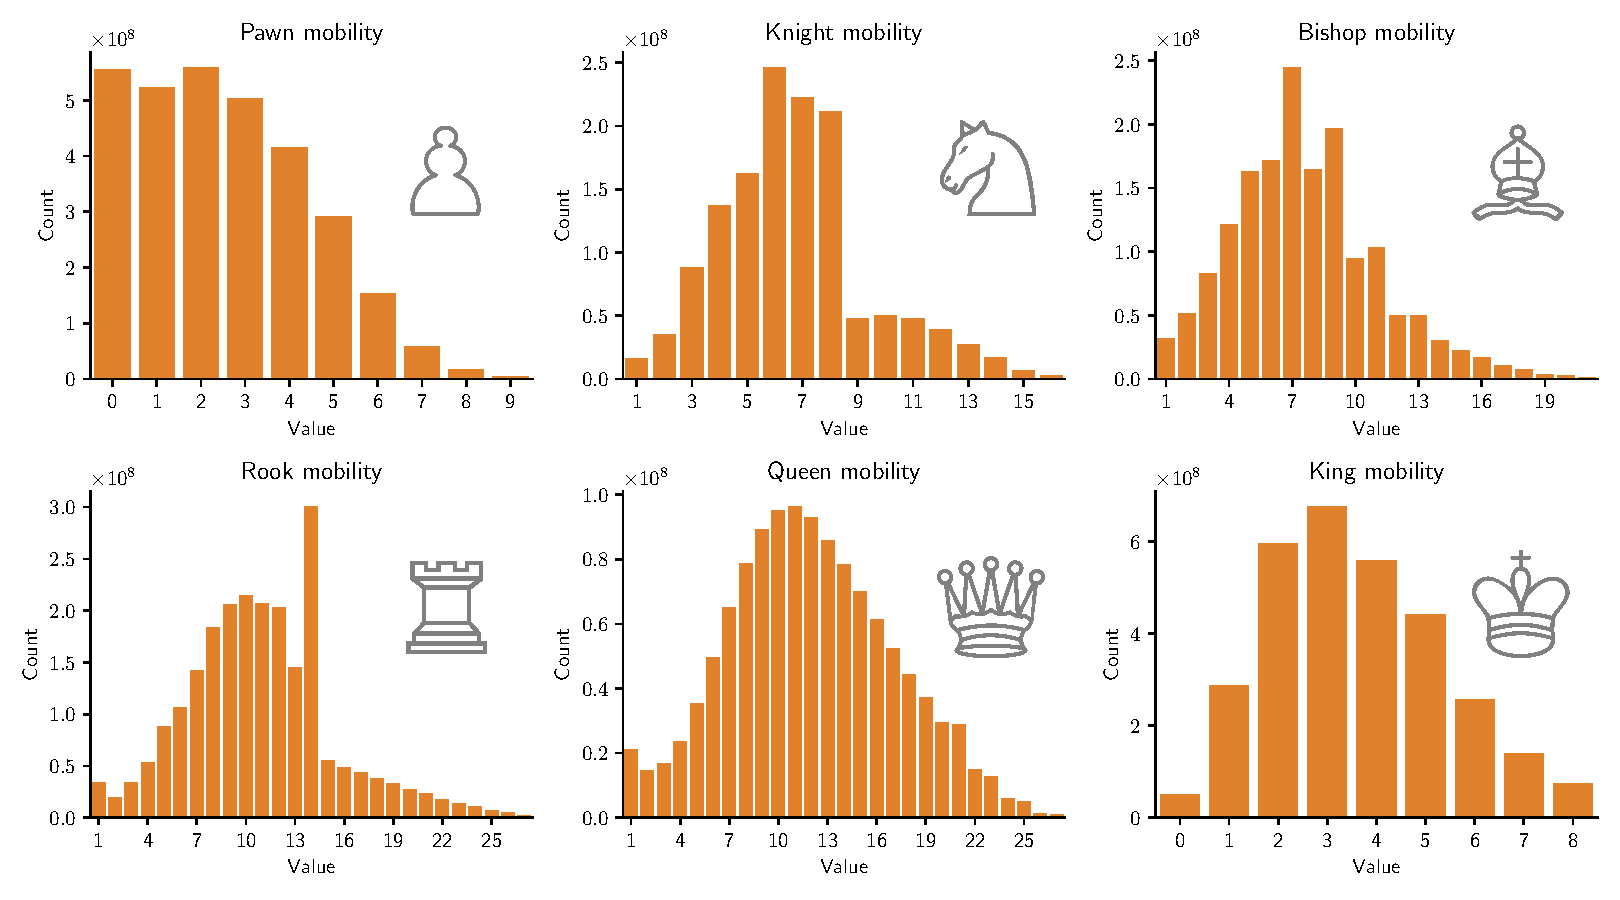
\includegraphics[width=\textwidth]{./dynamic/output/mobility.pdf}}
\caption{Total mobility values for each piece on the board. Computed using 2 billion boards. The value 0 for the \symknight\ Knight, \symbishop\ Bishop, \symrook\ Rook, and \symqueen\ Queen has been excluded from the plot, as it is very common.}
\label{fig:mobility}
\end{figure}
\end{itemize}

Each approach was implemented as a block:

\begin{table}[H]
\caption{Mobility feature blocks}
\label{tab:mobility_blocks}
\centering

\begin{tabular}{ccc}
\toprule
\bf Block name & \bf Definition & \bf Number of features \\
\toprule
MB & \makecell{
\vspace{0.2cm}
($\featureset{Squares} \times \featureset{Roles} \times \featureset{Colors})_P$ \\
P($\langle s, r, c \rangle$): there is a piece of role $r$\\ and color $c$ that \textbf{can move to} square $s$
} & 768 \\
\toprule
MC & \makecell{
\vspace{0.2cm}
$(\{0, 1, \hdots\} \times \featureset{Roles} \times \featureset{Colors})_{P}$\\
P($\langle m, r, c \rangle$): the value of mobility for\\
a piece of role $r$ and color $c$ is $m$
} & 206 \\
\bottomrule
\end{tabular}
\end{table}

The blocks will be combined with the \featureset{All} feature set. Neither of the blocks can be used alone since they do not carry the information to deduce every piece on the board (trivially).

The feature sets to be trained and evaluated are \featureset{All} $\oplus$ \featureset{MB} (1536 features) and \featureset{All} $\oplus$ \featureset{MC} (974 features). Like prior experiments, a network will be trained for each feature set and evaluated in a tournament. \\

\textbf{Results.} The results in table \ref{tab:mobility_results} show that the blocks did not provide features of enough quality to improve the network predictions enough to overcome the cost of making more feature updates. I have underestimated the cost of a feature update; that was not a problem in previous experiments. The block \featureset{MB} has, on average, 10.03 feature updates per move on average, and the block \featureset{MC} has 3.82 (see Appendix \ref{appendix:fs}). In comparison, the \featureset{All} feature set has 1.58 feature updates per move on average. Even though the block \featureset{MB} has almost 3 times the number of feature updates, it has better performance than \featureset{MC}. This is attributed to having a 7\% lower loss, which compensates the cost of the updates. \\

\begin{table}[H]
\caption{Mobility encodings results}
\label{tab:mobility_results}
\centering

\begin{tabular}{ccccc}
\toprule
\bf Feature set  & \bf \makecell{Number\\of features} & \makecell{\bf Val. loss\\\textit{min}} & \makecell{\bf Rating\\\textit{elo (rel. to \featureset{All})}} \\
\toprule
\featureset{All} (reference) & 768 & 0.003134 & \textbf{0.0} \\
\midrule
\featureset{All} $\oplus$ \featureset{MB} & 1536 & 0.002824 & -260.9 $\pm$ 5.4 \\
\midrule
\featureset{All} $\oplus$ \featureset{MC} & 974 & 0.003032 & -280.9 $\pm$ 5.6 \\
\bottomrule
\end{tabular}
\end{table}
